% Native original images; exact positions and crops are in the companion JSON.
\begin{figure*}[t]
\centering
\begingroup
\rmfamily
\setlength{\unitlength}{\dimexpr\linewidth/495\relax}
\begin{picture}(495,163)
\put(136.500,154.500){\makebox(0,0)[c]{\fontsize{8.5}{9.5}\selectfont\bfseries\color[HTML]{222222}Visit 1}}
\put(376.500,154.500){\makebox(0,0)[c]{\fontsize{8.5}{9.5}\selectfont\bfseries\color[HTML]{222222}Visit 2}}
\put(18.000,150.000){\color[HTML]{b9b9b9}\rule{237.000\unitlength}{0.5pt}}
\put(258.000,150.000){\color[HTML]{b9b9b9}\rule{237.000\unitlength}{0.5pt}}
\put(76.500,138.500){\makebox(0,0)[c]{\fontsize{7.5}{8.5}\selectfont\color[HTML]{222222}80 s}}
\put(18.000,68.962){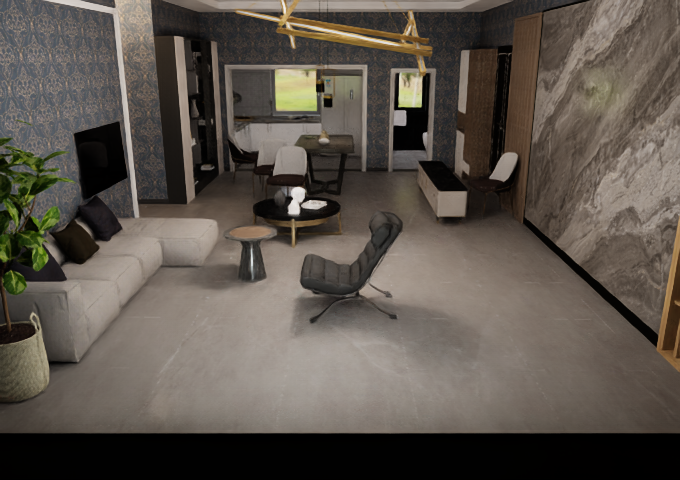
\includegraphics[width=117.000\unitlength,trim={0.0000bp 92.0000bp 0.0000bp 10.0000bp},clip]{figures/results_native/temporal/1_visit1_080s/0_gt.png}}
\put(18.000,1.962){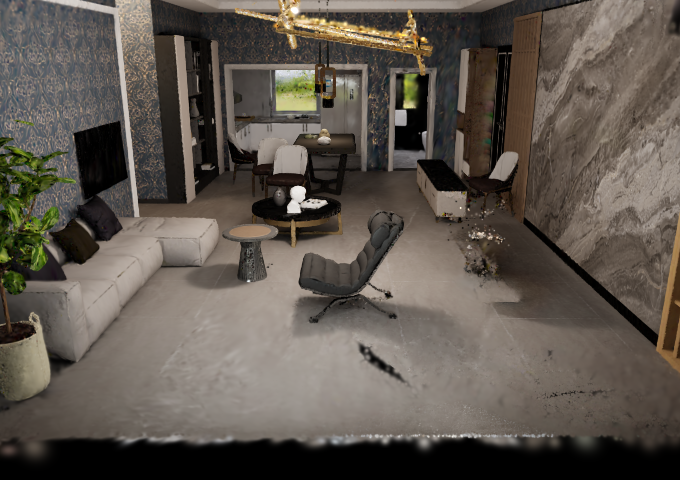
\includegraphics[width=117.000\unitlength,trim={0.0000bp 92.0000bp 0.0000bp 10.0000bp},clip]{figures/results_native/temporal/1_visit1_080s/5_ours_3dgs.png}}
\put(196.500,138.500){\makebox(0,0)[c]{\fontsize{7.5}{8.5}\selectfont\color[HTML]{222222}End}}
\put(138.000,68.962){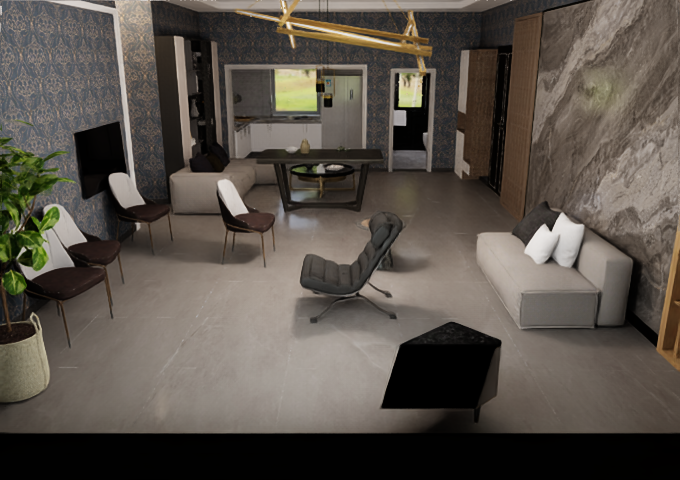
\includegraphics[width=117.000\unitlength,trim={0.0000bp 92.0000bp 0.0000bp 10.0000bp},clip]{figures/results_native/temporal/2_visit1_end/0_gt.png}}
\put(138.000,1.962){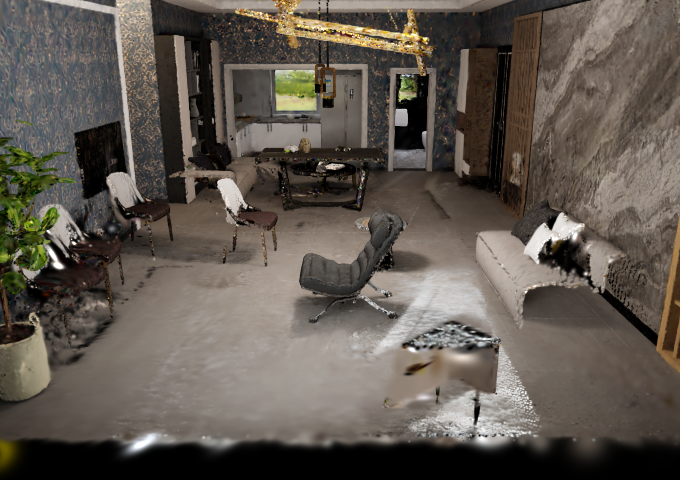
\includegraphics[width=117.000\unitlength,trim={0.0000bp 92.0000bp 0.0000bp 10.0000bp},clip]{figures/results_native/temporal/2_visit1_end/5_ours_3dgs.png}}
\put(316.500,138.500){\makebox(0,0)[c]{\fontsize{7.5}{8.5}\selectfont\color[HTML]{222222}97 s}}
\put(258.000,68.962){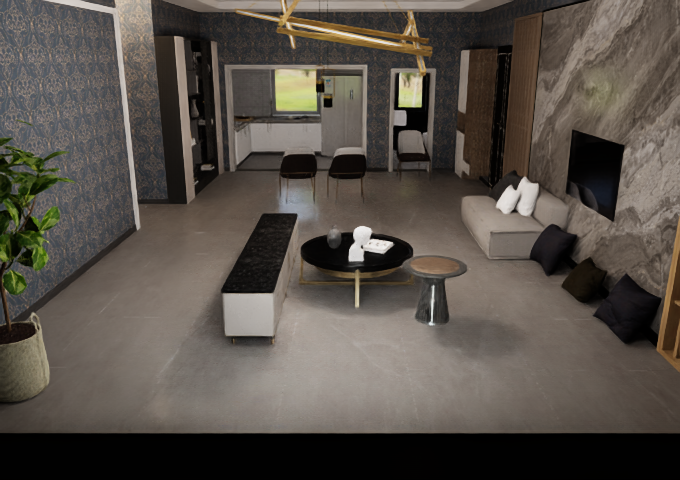
\includegraphics[width=117.000\unitlength,trim={0.0000bp 92.0000bp 0.0000bp 10.0000bp},clip]{figures/results_native/temporal/3_visit2_097s/0_gt.png}}
\put(258.000,1.962){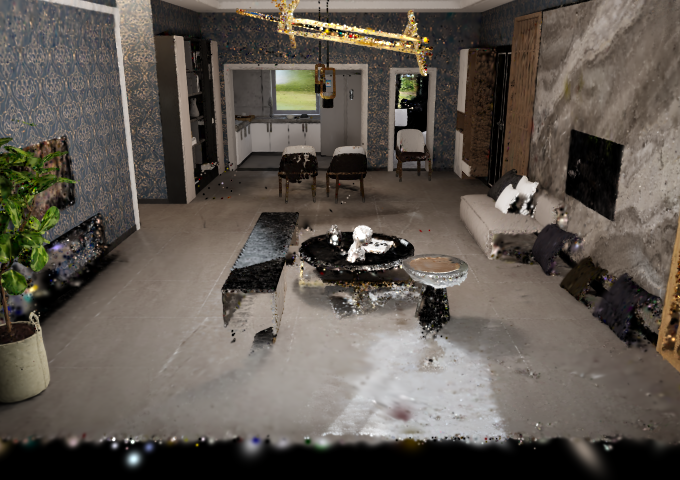
\includegraphics[width=117.000\unitlength,trim={0.0000bp 92.0000bp 0.0000bp 10.0000bp},clip]{figures/results_native/temporal/3_visit2_097s/5_ours_3dgs.png}}
\put(436.500,138.500){\makebox(0,0)[c]{\fontsize{7.5}{8.5}\selectfont\color[HTML]{222222}End}}
\put(378.000,68.962){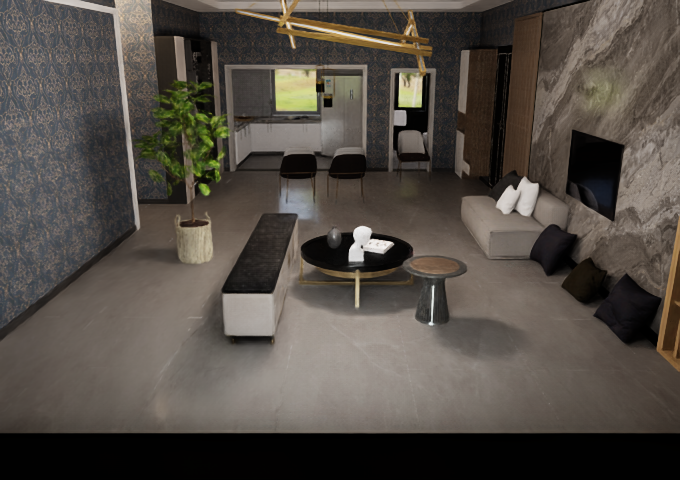
\includegraphics[width=117.000\unitlength,trim={0.0000bp 92.0000bp 0.0000bp 10.0000bp},clip]{figures/results_native/temporal/4_visit2_end/0_gt.png}}
\put(378.000,1.962){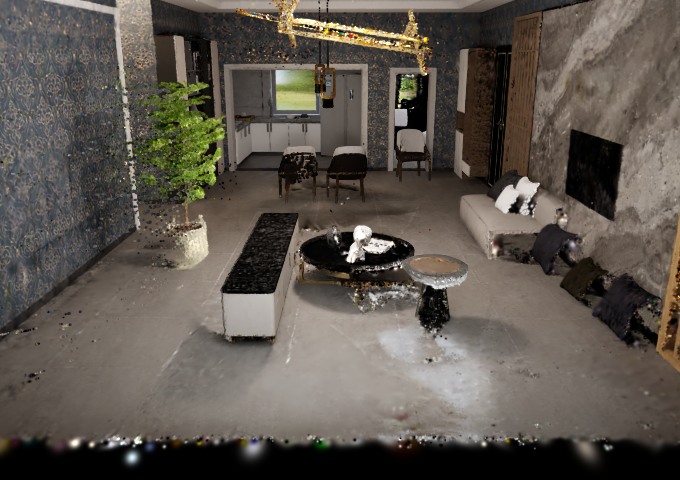
\includegraphics[width=117.000\unitlength,trim={0.0000bp 92.0000bp 0.0000bp 10.0000bp},clip]{figures/results_native/temporal/4_visit2_end/5_ours_3dgs.png}}
\put(256.500,132.000){\color[HTML]{888888}\rule{0.45pt}{2.000\unitlength}}
\put(256.500,127.000){\color[HTML]{888888}\rule{0.45pt}{2.000\unitlength}}
\put(256.500,122.000){\color[HTML]{888888}\rule{0.45pt}{2.000\unitlength}}
\put(256.500,117.000){\color[HTML]{888888}\rule{0.45pt}{2.000\unitlength}}
\put(256.500,112.000){\color[HTML]{888888}\rule{0.45pt}{2.000\unitlength}}
\put(256.500,107.000){\color[HTML]{888888}\rule{0.45pt}{2.000\unitlength}}
\put(256.500,102.000){\color[HTML]{888888}\rule{0.45pt}{2.000\unitlength}}
\put(256.500,97.000){\color[HTML]{888888}\rule{0.45pt}{2.000\unitlength}}
\put(256.500,92.000){\color[HTML]{888888}\rule{0.45pt}{2.000\unitlength}}
\put(256.500,87.000){\color[HTML]{888888}\rule{0.45pt}{2.000\unitlength}}
\put(256.500,82.000){\color[HTML]{888888}\rule{0.45pt}{2.000\unitlength}}
\put(256.500,77.000){\color[HTML]{888888}\rule{0.45pt}{2.000\unitlength}}
\put(256.500,72.000){\color[HTML]{888888}\rule{0.45pt}{2.000\unitlength}}
\put(256.500,67.000){\color[HTML]{888888}\rule{0.45pt}{2.000\unitlength}}
\put(256.500,62.000){\color[HTML]{888888}\rule{0.45pt}{2.000\unitlength}}
\put(256.500,57.000){\color[HTML]{888888}\rule{0.45pt}{2.000\unitlength}}
\put(256.500,52.000){\color[HTML]{888888}\rule{0.45pt}{2.000\unitlength}}
\put(256.500,47.000){\color[HTML]{888888}\rule{0.45pt}{2.000\unitlength}}
\put(256.500,42.000){\color[HTML]{888888}\rule{0.45pt}{2.000\unitlength}}
\put(256.500,37.000){\color[HTML]{888888}\rule{0.45pt}{2.000\unitlength}}
\put(256.500,32.000){\color[HTML]{888888}\rule{0.45pt}{2.000\unitlength}}
\put(256.500,27.000){\color[HTML]{888888}\rule{0.45pt}{2.000\unitlength}}
\put(256.500,22.000){\color[HTML]{888888}\rule{0.45pt}{2.000\unitlength}}
\put(256.500,17.000){\color[HTML]{888888}\rule{0.45pt}{2.000\unitlength}}
\put(256.500,12.000){\color[HTML]{888888}\rule{0.45pt}{2.000\unitlength}}
\put(256.500,7.000){\color[HTML]{888888}\rule{0.45pt}{2.000\unitlength}}
\put(8.000,101.500){\makebox(0,0){\rotatebox{90}{\fontsize{8}{9}\selectfont\color[HTML]{222222}Reference}}}
\put(8.000,34.500){\makebox(0,0){\rotatebox{90}{\fontsize{8}{9}\selectfont\color[HTML]{997510}Ours (3DGS)}}}
\end{picture}
\endgroup
\caption{\textbf{Gaussian reconstruction within and across visits.} Columns follow one reconstruction through two visits; the dashed divider marks the visit boundary. Ground truth is rendered at the indicated time; maps use the next saved snapshot, with no intervening scene change. All panels share the camera and clipping plane.}
\label{fig:evolution}
\end{figure*}
